\chapter{Physical aspects}

Atomic nuclei have multiple energy states, many of which are not stable, forcing them to release some of their energy in order to reach a stable state. However, one decay does not always lead to a direct transition into a stable state, it may even require the atom to transform into another, depending on what way it has released its energy. The theory in this chapter regarding energy and particle emissions from decaying nuclei is based on the detailed information shown in the first chapters of ``Radiation Detection and Measurement'' by Glenn F. Knoll \cite{knoll2010radiation}. 

Radiation is not only produced when atoms decay, it is constantly raining down upon us from the cosmos, this kind of radiation can also be detected with a CosmicWatch and is currently its primary use scenario, making cosmic rays an important field of study while working with CosmicWatches. The section regarding cosmic rays and showers is greatly inspired by the contents of ``Cosmic Rays'' by Bruno Rossi \cite{brunoRossi} and the extensive ``Review of Particle Physics'' \cite{ReviewOfParticlePhysics}. This chapter thus aims to provide an overview of the radiation to which CosmicWatch is sensitive and some of its production mechanisms. Chapter \ref{chap:detection_methods} provides an overview of how this can be used to take interesting measurements with CosmicWatch.

\section{Radioactivity}

It is first necessary to understand the concept of activity. Not all atoms take the same time to decay, each atom has its own constant $\Gamma$ which determines how likely it is to decay per unit of time. If one has an initial total of $N_0$ atoms, after a while it will be reduced due to the constant decay of atoms in the sample, this rate of change is given by the universal law of radioactive decay.
\begin{equation}
    \frac{dN(t)}{dt} = -\Gamma N(t)
\end{equation}

From this, it is easy to find that the number of remaining unstable atoms follows an exponential law
\begin{equation}
    N(t) = N_0 e^{-\Gamma t}
\end{equation}

The activity $A(t)$ of a radioactive source is given by how many decays occur per unit of time. This can be therefore obtained by multiplying the number of atoms $N(t)$ by the probability of decay per unit of time $\Gamma$.
\begin{equation}
    A(t) = \Gamma N_0 e^{-\Gamma t}
\end{equation}

The most common units for activity are the \textit{curie} (Ci) and the \textit{becquerel} (Bq), a becquerel represents one disintegration per second, while a curie represents $3.7\times10^{10}$ disintegrations per second ($\approx$ the activity of one gram of $^{226}Ra$). Under these definitions, the conversion between these units is given by the following relation:
\begin{eqnarray}
    1 \text{~Bq} = 2.703\times10^{-11} \text{~Ci}
\end{eqnarray}

The time constant $\Gamma$ is often expressed in terms of the atom's lifetime $\tau$ under the relation $\Gamma=1/\tau$. This means that $\tau$ is the time it takes to reduce a sample of $N_0$ by a factor of $1/e$, clearly $N(\tau)=N_0e^{-\Gamma \tau} = N_0/e$. On the other hand there also exists a constant called half-life $T_{1/2}$, which represents the time it takes to reduce the sample by half, Sodium 22 for example has a half-life of 2.605 years. They can both be related by doing $T_{1/2} = \ln (2)\tau$.

\subsection{Gamma emission}

\begin{figure}
  \centering
  \begin{subfigure}[t]{0.45\textwidth}
    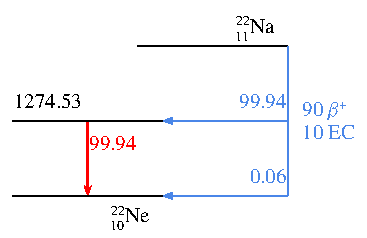
\includegraphics[width=\textwidth]{physical_aspects/22Na-decay.pdf}
    \caption{\label{sfig:22Na}}
  \end{subfigure}
  \begin{subfigure}[t]{0.425\textwidth}
    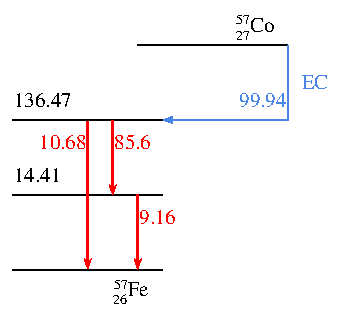
\includegraphics[width=\textwidth]{physical_aspects/57Co-decay.pdf}
    \caption{\label{sfig:57Co}}
  \end{subfigure}
  \medskip
  \centering
  \begin{subfigure}[t]{0.425\textwidth}
    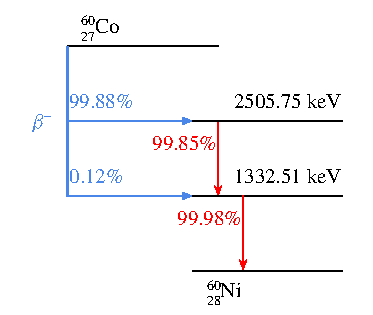
\includegraphics[width=\textwidth]{physical_aspects/60Co-decay.pdf}
    \caption{\label{sfig:60Co}}
  \end{subfigure}
  \begin{subfigure}[t]{0.425\textwidth}
    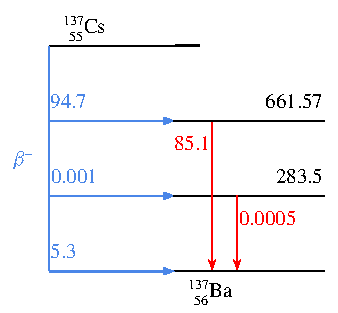
\includegraphics[width=\textwidth]{physical_aspects/137Cs-decay.pdf}
    \caption{\label{sfig:137Cs}}
  \end{subfigure}
  \caption{\label{fig:decay_schemes}Decay schemes for some isotopes used while testing the CosmicWatch. Only the main decay channels are included for clarity and simplicity. Energies [\unit{\kilo\eV}] for every level are shown in black. Branching ratios and decay mechanisms are shown in \textcolor{blue}{blue}. Gamma decays are represented with a \textcolor{red}{red} arrow also with its corresponding branching ratio.}
\end{figure}

Unstable nuclei have multiple channels to release their energy through, the conditions that determine what channels an atom can use are not studied here, but rather the subsequent effects of such channels. An atom can decay by emitting gamma rays, alpha particles, neutrons, or protons, it can also undergo beta $\beta^{\pm}$ decay, Internal Conversion, and Electron Capture among others. This work will focus on beta decay and Electron Capture since these are the preferred channels of decay of the radioactive sources used to test CosmicWatch.

\subsubsection{Beta decay} \label{sec:beta_decay}

There are two types of beta decay, they are represented by the following reaction schemes:
\begin{align}
  \beta^+ &:=~ ^A_ZX \rightarrow ~ ^A_{Z-1}Y + e^+ + \nu \\
  \beta^- &:=~ ^A_ZX \rightarrow ~ ^A_{Z+1}Y + e^- + \bar{\nu}
\end{align}

Where the symbols follow the nuclear notation, $X$ and $Y$ represent the initial and final elements, $A$ is the atomic number, $Z$ the nuclear charge, $e^{\pm}$ are a positron or electron, and $\nu/\bar{\nu}$ are a neutrino/antineutrino, Fig. \ref{fig:decay_schemes} shows some examples of these processes. Note for instance the case of $^{22}_{11}$Na Fig. \ref{sfig:22Na}, it undergoes $\beta^+$ $90\%$ of the time it decays, by the nuclear notation one can tell that the initial and final elements are Sodium and Neon respectively. In this process, a proton turns into a neutron, which is why the product element has $Z=11-1=10$ while maintaining $A=22$. It is important to also note that the total charge has to be conserved after the reaction occurs, which is why a positron $e^+$ is produced.

Alongside the positron/electron, a neutrino/antineutrino is ejected from the nucleus which, due to its extremely small interaction probability with matter, can not be detected. However, the negligible neutrino/antineutrino-matter interactions do not mean that their presence in the reaction does not have effects. The energy of the system also has to be conserved, since the particles $e^{\pm}$ and $\nu/\bar{\nu}$ are all ejected from the nucleus, higher or smaller portions of the total energy can be taken by the neutrino/antineutrino, which leaves multiple possible energy values for the positron/electron, resulting in continuous energy spectra.

\begin{figure}[H]
    \centering
    \begin{subfigure}[t]{0.45\textwidth}
      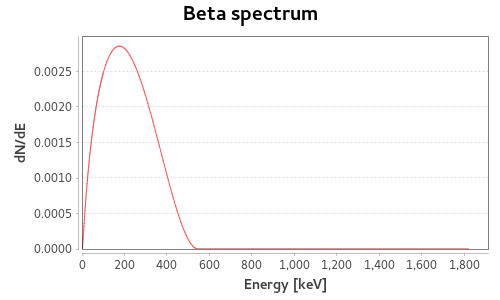
\includegraphics[width=\textwidth]{physical_aspects/22Na-beta-spectrum.jpg}
      \caption{\label{sfig:22Na_beta_spectra}}
    \end{subfigure}
    \begin{subfigure}[t]{0.45\textwidth}
      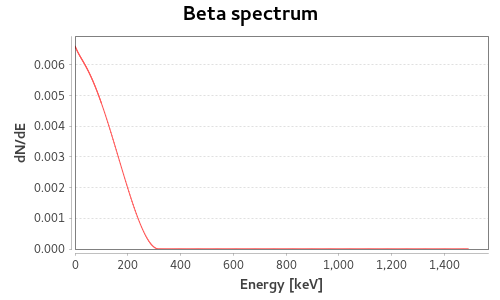
\includegraphics[width=\textwidth]{physical_aspects/60Co-beta-spectrum.jpg}
      \caption{\label{sfig:60Co_beta_spectra}}
    \end{subfigure}
    \caption{\label{fig:beta_spectra}positron/electron energy spectra for  \subref{sfig:22Na_beta_spectra} $^{22}$Na $(\beta^+)$ and  \subref{sfig:60Co_beta_spectra} $^{60}$Co $(\beta^-)$. Taken from \cite{IAEA}.}
\end{figure}

\subsubsection{LYSO self-radiation}\label{sec:self_radiation}

\subsubsection{Electron Capture}

The process of Electron Capture is analogous to $\beta^+$ decay, here an electron from de $K$ shell (or $L$, $M$, \dots) is captured by a proton in the nucleus, which then turns into a neutron while emitting a neutrino with a characteristic energy. The effect of this decay in the nucleus is the same as in $\beta^+$: (Z, A)$\rightarrow$(Z-1, A). The decay scheme is represented below:

\begin{equation}
  \text{EC} :=~ p + e^- \rightarrow ~ n + \nu
\end{equation}

Since this process leaves a vacancy in the lower shells of the electron cloud, an electron in an upper shell can decay to fill the space, resulting in the emission of characteristic X-rays.

\subsection{Light-matter interactions}

This section shows a review of the most important processes that govern gamma-ray interactions with matter, them being the photoelectric effect, Compton scattering, and pair production.

\subsubsection{photoelectric effect}

This effect was first described by Albert Einstein in \cite{einstein1905heuristic}, it is the emission of electrons from an atom due to the absorption of light. The electrons are emitted with an energy close to that of the absorbed photon $E_\gamma$ and is given by equation \eqref{eq:photoelectric}
\begin{equation}
  E_{e^-} = E_\gamma - E_b \label{eq:photoelectric}
\end{equation}
Where $E_b$ is the binding energy of the electron in the atom. $E_b$ will therefore depend on the electron's original shell since outer shells have lower binding energies.

\subsubsection{Compton scattering}\label{sec:compt_scattering}

\begin{figure}[H]
  \centering
  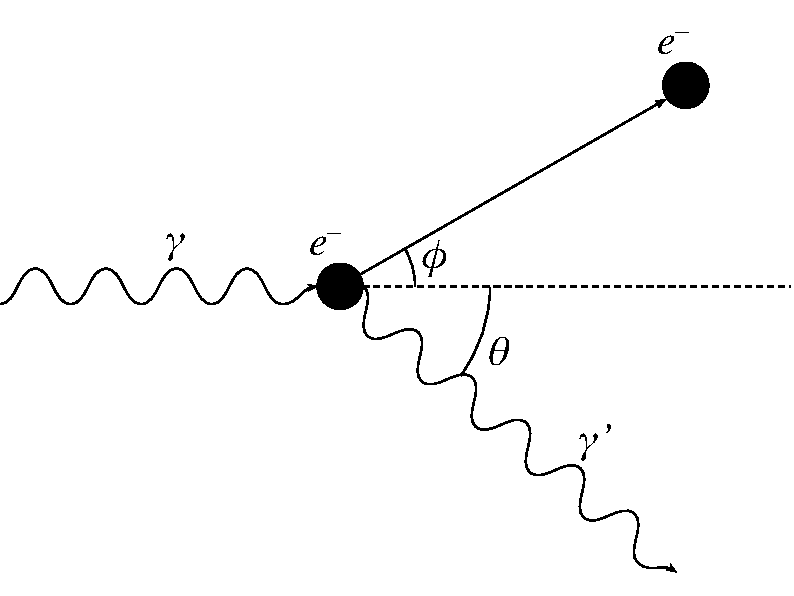
\includegraphics[width=.4\textwidth]{physical_aspects/Compton-scattering.pdf}
  \caption{\label{fig:Compton_scattering_diagram}Gamma-ray Compton scattering diagram.}
\end{figure}

Compton scattering occurs most often when a photon interacts with an electron in the sensitive material, it can be understood as a collision between the two, where the electron is considered initially static and then gains part of the photon's energy $E_0$ after deflecting it. Fig \ref{fig:Compton_scattering_diagram} shows an example of a gamma ray being scattered by an electron, the recoil electron is ejected with an angle $\phi$ while the scattered gamma ray travels with an angle $\theta$. It can be shown that the energy of the scattered photon $E_{1}$ and the recoil electron $E_e$ follow equations \eqref{eq:compton}
\begin{align}
  E_{1} &= \frac{E_0}{1+\epsilon(1-\cos\theta)} \label{eq:compton},~ & E_e &= E_0 - E_1 = E_0\frac{\epsilon(1-\cos\theta)}{1+\epsilon(1-\cos\theta)},~ & \epsilon&=\frac{E_0}{m_{e}c^2} 
\end{align}
where $m_e c^2$ is the resting energy of the electron (511 \unit{\kilo\eV}). It is easy to see that high scattering angles greatly reduce the photon's energy, meaning that $E_e$ will be higher. For $\theta=\pi$ and $\phi=0$, it is therefore clear that the electron will gain the maximum energy possible, which is lower than $E_0$, this will be important while detecting gammas since photomultipliers collect the energy carried by electrons, which is further explored in Chapter \ref{chap:detection_methods}.

\subsubsection{Pair production}

This effect is the creation of a particle and its antiparticle from a neutral boson, most often referred to when an electron and a positron are produced by a photon. In order for this to occur, the initial photon's energy needs to be higher than that of the resting pair ($2m_e c^2=1022$ \unit{\kilo\eV}), any exceeding energy will turn into kinetic energy for the pair.

In the case of $^{22}$Na, as shown in Fig. \ref{sfig:22Na}, there is a transition from an excited state of $^{22}$Ne which emits a 1274.53 \unit{\kilo\eV} gamma, making pair production possible. Electron-positron annihilation is therefore a byproduct of this decay, making it important while studying its spectra.

\begin{figure}[H]
  \centering
  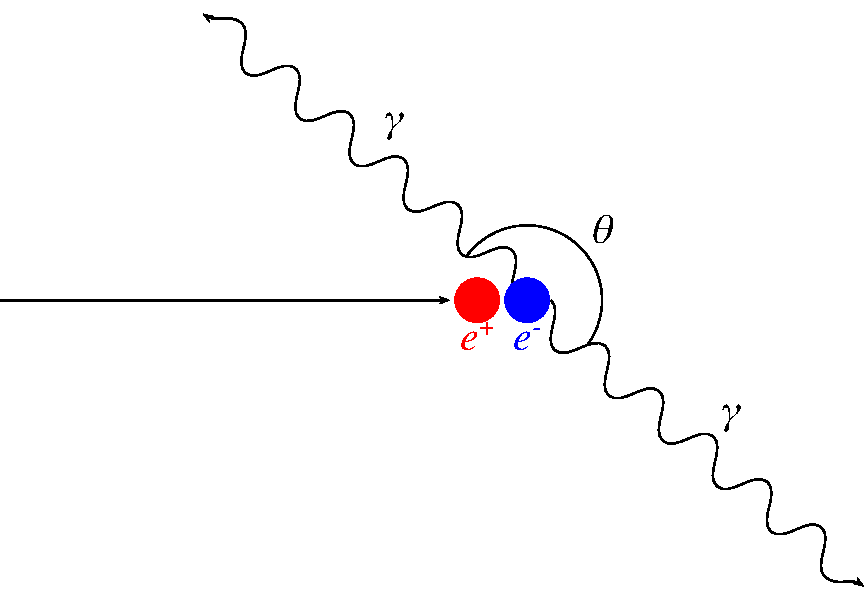
\includegraphics[width=.5\textwidth]{physical_aspects/positron-annihilation.pdf}
  \caption{\label{fig:positron_annihilation_diagram}Electron-positron annihilation diagram.}
\end{figure}

Once the positron produced by pair production slows down, it will most probably annihilate with an electron in the medium, producing two oppositely traveling gammas both with energy 511 \unit{\kilo\eV}, which combined is equal to the resting masses of both particles (1022 \unit{\kilo\eV}).

\subsection{Gammas inside the detector}

The light-matter interactions discussed in the previous subsection lead to different effects inside the detector that can be seen while measuring spectra. This subsection deals with some of the features that one should look for in a spectrum at the moment of calibrating the detector.

\begin{figure}[H]
  \centering
  \begin{subfigure}[t]{0.7\textwidth}
    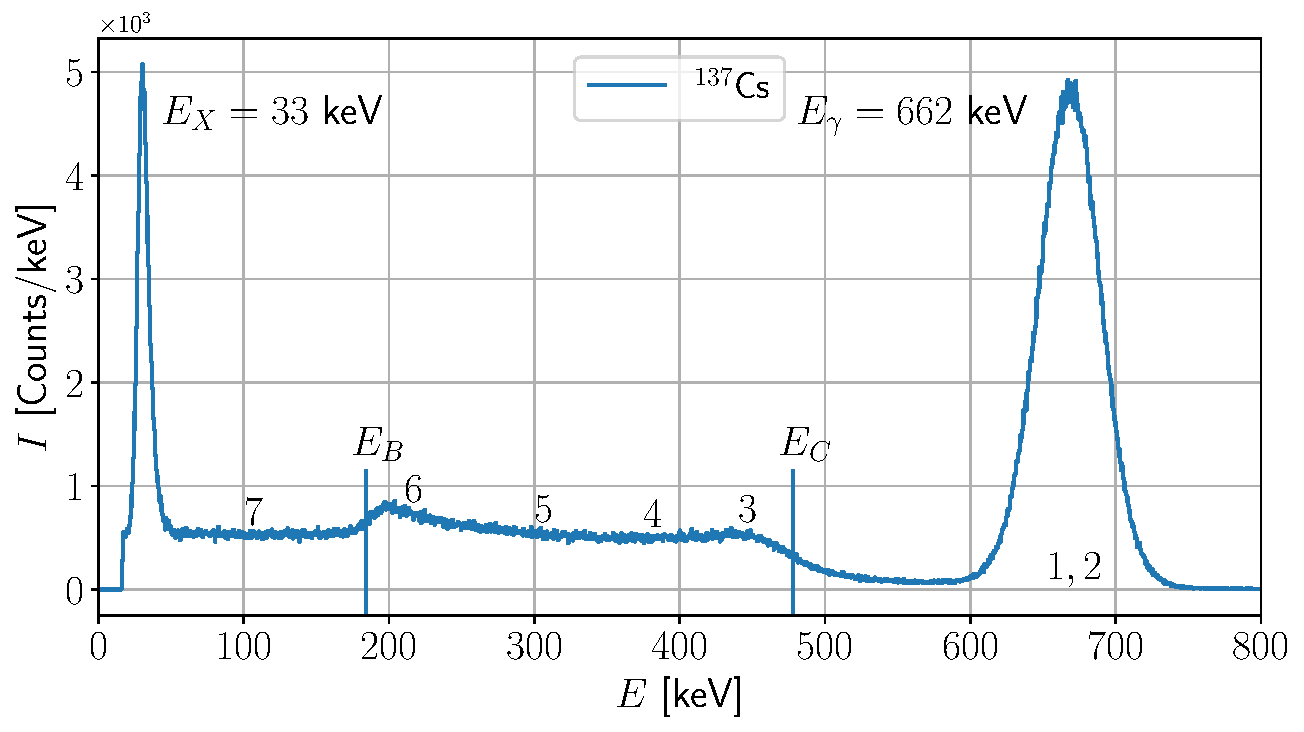
\includegraphics[height=6.3cm]{physical_aspects/energiesCs137.pdf}
    \caption{\label{sfig:spectrum_description}}
  \end{subfigure}
  \hfill
  \begin{subfigure}[t]{0.28\textwidth}
    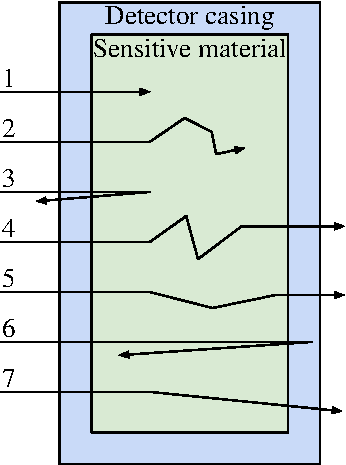
\includegraphics[height=6cm]{physical_aspects/gamma_interactions.pdf}
    \caption{\label{sfig:gamma_scattering}}
  \end{subfigure}
  \caption{\label{fig:Cs137_description}$^{137}$Cs spectrum highlighting some of the main features that commonly appear in gamma-ray spectra. Black arrows in \subref{sfig:gamma_scattering} represent detected gamma rays, changes in direction are due to Compton scattering. A detailed discussion about the meaning of these processes is given below. Adapted from \cite{Notas-instrumentacion}.}
\end{figure}

As discussed in subsection \ref{sec:compt_scattering}, incident gamma rays can be deflected by electrons inside the detector in various ways, therefore, the electron energy that will ultimately be detected is not always the same. For example, a gamma ray can deposit all of its energy by being photoelectrically absorbed directly (1 in Fig. \ref{sfig:gamma_scattering}), or, after undergoing multiple Compton scatterings $(2)$. Fractions of the total energy can also be detected since gammas can Compton-scatter multiple times and then escape the detector $(3, 4, 5, 7)$. This is known as Compton background, and can also be used to differentiate radioactive isotopes in gamma spectroscopy.

There are some energies worth noting since they give the Compton background a recognizable shape. They are known as the backscattering and Compton edge energies and their origins are discussed next.

\subsubsection{Compton edge}

Theoretically, the maximum energy a gamma ray can transfer to an electron, according to \eqref{eq:compton}, occurs when the photon is deflected with $\theta=\pi$, this is called the Compton edge, represented here as $E_C$ $(3)$, since no electron should gain energies between $E_C$ and the photoelectric energy.
\begin{equation}
  E_C=E_{e\text{max}}=E_0\frac{2\varepsilon}{1+2\varepsilon}
\end{equation}

\subsubsection{backscattering}
On the other hand, relatively small energies can also be transferred by gammas to electrons in the detector. This happens when the casing scatters a gamma which is then absorbed inside the sensitive material $(6)$. In this case, the energy deposition is also given by \eqref{eq:compton} but will depend on the backscattering angle:
\begin{equation}
    E_B=E_1=\frac{E_0}{1+\varepsilon(1-\cos\theta)}
\end{equation}

\section{Cosmic Radiation}

Cosmic rays are high-energy particles and clusters of particles originating from all around the universe. Cosmic rays are constantly raining down upon us, but the Earth's atmosphere and magnetic field protect us by reducing their energy and deflecting them. However, through various processes, some of these particles can produce new which are now capable of reaching sea level. CosmicWatches can also be used to measure some of these particles and their properties, making them worth studying here.

The particles that initially reach the atmosphere are known as primaries, protons and bare nuclei of heavier elements make up for most of them. Once the primaries reach the atmosphere they interact with oxygen and hydrogen molecules, breaking them apart and producing new particles that will further interact with the atmosphere, creating what is known as a cosmic ray shower. A simplified diagram of cosmic ray showers is shown in Fig. \ref{fig:cosmic-shower-diagram}.

\begin{figure}
\centering
\begin{tikzpicture}[scale=0.9]
  \tikzset{edge from parent/.style=
  {draw,
  edge from parent path={(\tikzparentnode.south)
  -- +(0,-8pt)
  -| (\tikzchildnode)}}}
  \Tree [.{primary}
  [.{Nuclear collision} 
    [.$p$ 
      [.{Hadronic cascade} 
        [.$\pi^{\pm}$ \edge[dashed] node[]{}; [.{} ] ]
        [.$\pi^0$ \edge[dashed] node[]{}; [.{} ] ]
        [.$p(\bar{p})$ \edge[dashed] node[]{}; [.{} ] ]
        [.$n(\bar{n})$ \edge[dashed] node[]{}; [.{} ] ]
        [.$K^{\pm}$ \edge[dashed] node[]{}; [.{} ] ]
        [.$K^{0}$ \edge[dashed] node[]{}; [.{} ] ]
      ]
    ]
    [.$\pi^0$
      [.{Decay} 
        [.$\gamma$ 
          [.{Pair production}
            [.$e^+$ 
              [.{Bremsstrahlung}
                [.$\gamma$ 
                  [.$e^-$ ]
                  [.$e^+$ ]
                ]
                [.$e^+$ 
                  [.$\gamma$ ]
                  [.$e^+$ ]
                ]
              ]
            ]
            [.$e^-$ \edge[dashed] node[]{}; [.{} ] ]
          ]
        ]
        [.$\gamma$ 
          [.$e^-$ \edge[dashed] node[]{}; [.{} ] ]
          [.$e^+$ \edge[dashed] node[]{}; [.{} ] ]
        ]
      ] 
    ]
    [.$\pi^{\pm}$
      [.{Decay} 
        [.$\mu^{\pm}$ 
          [.{Decay} 
            [.$e^{\pm}$ ]
            [.$\nu$ ]
            [.$\bar{\nu}$ ]
          ]
        ]
        [.$\nu$ ]
      ] 
    ]
    [.$\pi^{\pm}$
      [.{Hadronic cascade} 
        [.$\pi^{\pm}$ 
          [.$\mu^{\pm}$ ]
          [.$\nu(\bar{\nu})$ ]
        ]
        [.$\pi^0$ 
          [.$\gamma$ \edge[dashed] node[]{}; [.{} ] ]
          [.$\gamma$ \edge[dashed] node[]{}; [.{} ] ]
        ]
      ] 
    ]
  ] 
  ]
\end{tikzpicture}
\caption{Cosmic-ray shower evolution diagram. Adapted from \cite{brunoRossi}}
\label{fig:cosmic-shower-diagram}
\end{figure}

\section{Particle interactions with matter}

The type of interaction highly depends on the type of particle we are dealing with, as mentioned before for example, neutrinos interact very little with matter, making them invisible to CosmicWatches. Due to how light electrons and positions are $m_ec^2=0.511$ \unit{\mega\eV}, their trajectories can be easily modified due to electromagnetic interactions with surrounding atoms, while heavier particles can keep a ``straight'' trajectory depending on their energy. Muons are the particle with the lowest mass ($m_\mu c^2=105.7$  \unit{\mega\eV}) greater than the electron and it is still 200 times heavier, allowing us to divide particle interactions into those of ``light'' charged particles (electrons and positrons) or ``heavy'' charged particles. This section shows a brief explanation of some of the processes that particles undergo while traversing materials and depositing their energy. It is also important to note that the main interactions occur between the particle and the orbital electrons in the detector's material, particle-nuclei interaction may also occur, these are however much less common, which is why detectors rely on particle-electron interactions.

\subsection{Interactions of heavy charged particles}

\begin{figure}
  \centering
  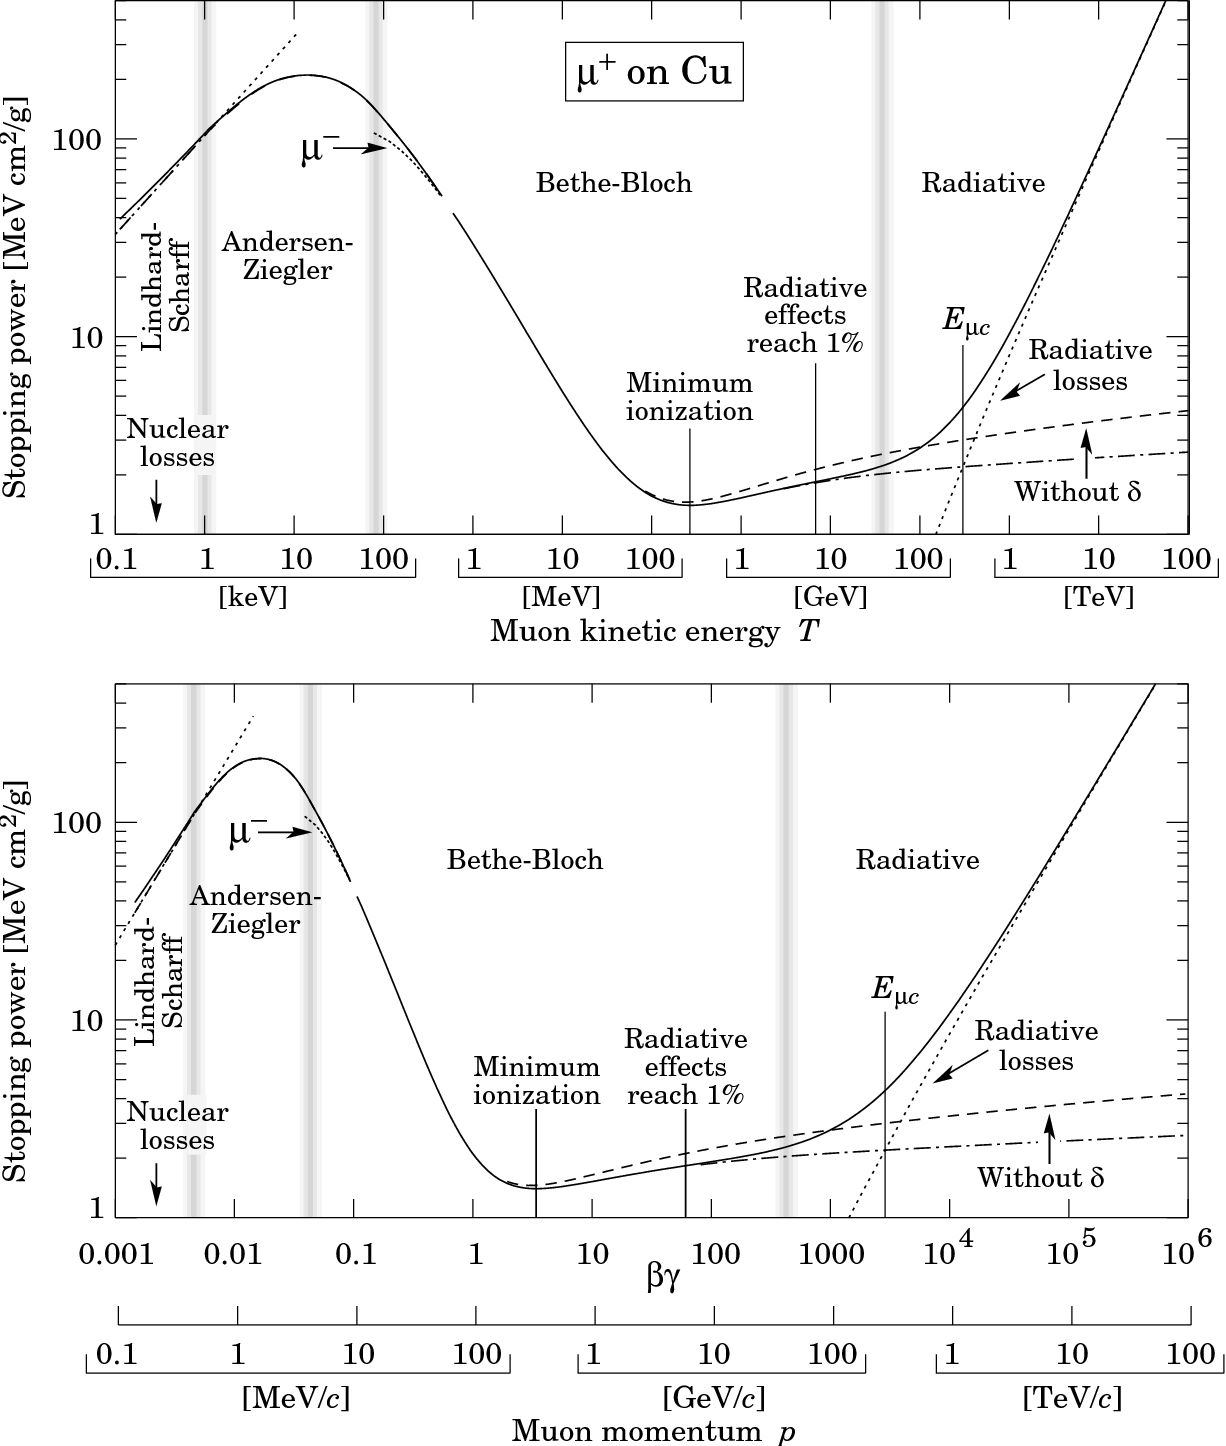
\includegraphics[width=.8\textwidth]{physical_aspects/muon_dEdx_copper.png}
  \caption{\label{fig:muon_dEdx}Muon stopping power from Bethe-Bloch equation with distinct adjustments for different energy/momentum ranges, taken from \cite{muon_dEdx}. A detailed discussion about the different energy ranges and interactions shown here can be found in \cite[sec.~32]{ReviewOfParticlePhysics}.}
\end{figure}

Once the charged particle has entered a medium, it transfers some of its energy to surrounding electrons, by either making them jump to a higher energy state (excitation) or removing them from the atom (ionization), depending on the strength of the interaction. The average energy loss per unit length traveled is known as the \textit{stopping power} $-dE/dx$, depending on the particle's energy the effects that induce the energy transfer will differ, which is why it can be divided into three regions. The limits of these regions depend on the effective atomic number of the absorber and the mass of the slowing particle \cite{ReviewOfParticlePhysics}, making them specific for every use case scenario. Figure \ref{fig:muon_dEdx} shows distinct regions where some interactions take the main role in the muon's energy loss.

\subsubsection{sub-relativistic region}

Here, particles have enough energy to remove orbiting electrons from the atom, and the energy loss increases with the distance traveled. In the case of positively charged particles, this may result in electron pickup, effectively decreasing its charge and therefore its electromagnetic interaction with the surrounding medium, making $-dE/dx$ fall off rapidly. The energy loss along a track is known as the Bragg curve, in the example discussed earlier it resembles a peak \cite{knoll2010radiation}.

\subsubsection{ionization region}

Atomic ionization and excitation take great importance in this region. The high velocities prevent particles from picking up electrons, maintaining their charge constant, and effectively losing energy by slowing down. The Bethe-Bloch formula gives a good approximation of the energy loss in this region (corrections are made for the other regions). Here, normally above $10^2$ MeV for heavy particles and 1 MeV for electrons/positrons, $-dE/dx$ reaches an almost constant minimum of about $2$ \unit{\mega\eV\per{\g\cm\squared}} for light materials \cite[p.~32]{knoll2010radiation}. At this minimum, particles are called ``minimum ionizing particles'' since their ionization potential is the lowest, allowing them to travel deeper into the material. Since most muons reaching sea level have energies of around 4 \unit{\giga\eV} \cite[p.~380]{ReviewOfParticlePhysics}, this region is particularly relevant for CosmicWatches, meaning that they are most likely to trigger the detector by ionization of the material.

\subsubsection{ultra-relativistic region}

In this regime pair production, Bremsstrahlung, and photonuclear contributions become important. The energy threshold for radiative processes to become significant occurs at several hundred \unit{\giga\eV} in the case of muons, it is known as critical energy and is defined as the energy at which radiative and ionization losses are equal. Figure \ref{fig:muon_dEdx} shows this energy with the label $E_{\mu c}$. Bremsstrahlung in particular results interesting in this region, it means ``breaking radiation'' in German, and it is the release of electromagnetic radiation due to the deflection/acceleration of particles while interacting with surrounding heavy nuclei.

\subsection{Interactions of light charged particles}

Electrons and positrons reaching the Earth's surface have energies around 1 \unit{\giga\eV} and make up a great part of the cosmic radiation at sea level. At this and higher energies, Bremsstrahlung dominates the electron's energy loss, producing gamma rays (as shown in Fig. \ref{fig:cosmic-shower-diagram}) that may lead to further pair production, creating a cycle that will only stop once the pair produced electrons/positrons go bellow their critical energies $E_{ec}$. 

While detecting muons, this electronic background may interfere, since electrons and positrons will be mistaken for muons. Remembering the discussion at the beginning of this chapter about how electrons can be easily deflected due to their extremely low mass, the muon miscount can be avoided by placing the detector under some solid material (such as concrete or any kind of roof), or by using two detectors looking for coincident events, since it would be very unlikely that an electron will deposit energy in both.

\subsection{Coisne squared law}

As mentioned before, particles lose some of their energy while traversing a determined length of material, it is therefore reasonable to expect the intensity of cosmic rays to vary with the direction of incidence, as some may have to travel through more material. The relative intensity of cosmic rays as a function zenith angle follows a cosine squared law, showing that, for example, muons raining directly downward $(\theta=0)$ are more likely to reach sea level, as they are the ones that traverse the least atmosphere, while muons traveling horizontally $(\theta=\pi/2)$ have to go through a lot more air in order to reach the observation point. This idea is better illustrated in Fig. TALES.